% questions.tex —— 1977 年·广东卷 · 题目内容片段（无答案）
% 由 tools/generate_projects.py 依来源总账自 1977/1977_数学真题_广东_试题.md 生成，勿手改（改源 MD 后重跑）


\gkpart{数学试题解（广东卷）}

\begin{gktip}
\textbf{来源说明}：本题面依据固定源 PDF《广东1977年高考数学试题解》第 1—5 页（书籍页码 103—107）逐题转录。固定源是题面与解答连排出现的扫描材料，不是无答案试卷；第一至七题原卷均附解答，本库答案与解析另行独立推导并与源解答对照复算。正式题为第一至七题（原卷题号用汉字“一”至“七”，本库统一改为阿拉伯数字），末尾“参考题”两题原卷注明“在完成必答题以后，如时间允许，可以选做”，不计入题量、亦未印分值。原卷分值：第一题 22 分、第二题 10 分、第三题 16 分、第四题 10 分、第五题 12 分，第六、七题未印分值。文件名标注“含今海南省”（1977 年海南行政区属广东省）；原卷三角函数记号用 tg、ctg，对数记号用 Lg，题面按原样保留。
\end{gktip}

\par\medskip

\begin{question}
\gkti{1}\textbf{（22 分）} 计算：

（1） $(-3)^2-\left(-1\dfrac{1}{2}\right)^3\times\dfrac{2}{9}-6\div\left|-\dfrac{2}{3}\right|$；

（2） $\dfrac{x^2+2x+1}{x^3-x}\cdot\dfrac{x}{x+1}-\dfrac{1}{x+1}$；

（3） $\dfrac{\sqrt{20}}{8}-\sqrt{\dfrac{9}{5}}+\dfrac{5}{\sqrt{45}}$。

\end{question}
\begin{question}
\gkti{2}\textbf{（10 分）} 解方程：

\nopagebreak[4]
\[
\frac{x+3}{x+2}+\frac{x+1}{x-2}-1=0,
\]

并检验所得的结果是否是原方程的根。

\end{question}
\begin{question}
\gkti{3}\textbf{（16 分）} 计算：

（1） $\left(\dfrac{1}{2}\right)^{-1}-4\times(-2)^{-3}+\left(\dfrac{1}{2}\right)^{0}-9^{-\frac{1}{2}}$；

（2） $2\operatorname{Lg}a^{\frac{1}{3}}b^{2}-\operatorname{Lg}\dfrac{\sqrt{b}}{8}-3\operatorname{Lg}2$，其中 $\operatorname{Lg}a=0.33$，$\operatorname{Lg}b=0.22$。

\end{question}
\begin{question}
\gkti{4}\textbf{（10 分）} 证明恒等式：

\nopagebreak[4]
\[
\left(\frac{1}{\cos x}+1\right)\left(\frac{1}{\cos x}-1\right)\operatorname{ctg}x=\operatorname{tg}x.
\]

\Needspace{0.4\textheight}
\end{question}
\begin{question}
\gkti{5}\textbf{（12 分）} 已知小山上的电视发射塔 $AB$ 的高是 $50$ 米，自山下地面的 $C$ 点测得塔底 $B$ 的仰角是 $40^\circ$，塔顶 $A$ 的仰角是 $70^\circ$，求小山 $BD$ 的高。（精确到 $0.01$ 米，$\sin40^\circ=0.643$，$\sin20^\circ=0.342$）

\begin{gktip}
原源 PDF 第 3 页附有小山、发射塔与观测点 $C$ 的示意图；LaTeX 版按源图重绘。
\end{gktip}
\nopagebreak[4]
\begin{center}% 1977 年广东卷第 5 题：小山上的电视发射塔 AB（高 50 米），自山下地面 C 点测得
% 塔底 B 仰角 40°、塔顶 A 仰角 70°，D 在 B 正下方，右侧标 50 米尺寸线（按源卷第 3 页布局）
\begin{tikzpicture}[scale=0.75]
  % 地面
  \draw[thick] (-0.8,0) -- (9.8,0);
  % 小山轮廓
  \draw[thick] (1.6,0) .. controls (3.0,1.3) and (4.6,2.3) .. (6,3)
    .. controls (7.2,2.6) and (8.4,1.2) .. (9.4,0);
  \draw[thin] (3.6,0.9) .. controls (4.2,1.5) and (4.8,1.9) .. (5.4,2.4);
  \draw[thin] (6.6,2.4) .. controls (7.2,1.9) and (7.8,1.2) .. (8.2,0.5);
  % 发射塔（梯形塔身加交叉撑）
  \draw[thick] (5.75,3) -- (5.9,5.3) -- (6.1,5.3) -- (6.25,3) -- cycle;
  \draw[thin] (5.79,3.3) -- (6.21,3.9);
  \draw[thin] (6.21,3.3) -- (5.79,3.9);
  \draw[thin] (5.80,3.9) -- (6.20,4.5);
  \draw[thin] (6.20,3.9) -- (5.80,4.5);
  \draw[thin] (5.82,4.5) -- (6.18,5.1);
  \draw[thin] (6.18,4.5) -- (5.82,5.1);
  % 视线（虚线）
  \draw[dashed] (0,0) -- (6,5.3);
  \draw[dashed] (0,0) -- (6,3);
  \draw[dashed] (6,3) -- (6,0);
  % C 处两个仰角弧
  \draw (1.3,0) arc (0:26.57:1.3);
  \draw (1.85,0) arc (0:41.4:1.85);
  \node at (1.5,0.32) {$40^\circ$};
  \node at (1.62,1.05) {$70^\circ$};
  % 50 米尺寸线
  \draw[thin] (6.15,5.3) -- (8.7,5.3);
  \draw[thin] (6.35,3) -- (8.7,3);
  \draw[<->] (8.35,3) -- (8.35,5.3);
  \node[rotate=90] at (8.05,4.15) {50米};
  % 顶点标注
  \fill (6,5.3) circle (1.2pt) node[above] {$A$};
  \fill (6,3) circle (1.2pt) node[right=2pt] {$B$};
  \fill (0,0) circle (1.2pt) node[below] {$C$};
  \fill (6,0) circle (1.2pt) node[below] {$D$};
\end{tikzpicture}
\end{center}
\nopagebreak[4]
\Needspace{0.4\textheight}
\end{question}
\begin{question}
\gkti{6}如图，已知 $AE$ 和 $AF$ 是 $\odot O$ 的切线，$M\text{、}N$ 是切点，$EF$ 过圆心且垂直于 $AO$。求证：$AE=AF$。

\begin{gktip}
原源 PDF 第 3 页附有圆与切线示意图；LaTeX 版按源图重绘。
\end{gktip}
\nopagebreak[4]
\begin{center}% 1977 年广东卷第 6 题：AE、AF 切圆 O 于 M、N，直径 EF 过圆心 O 且垂直于 AO，
% OM、ON 画虚线（按源卷第 3 页布局）
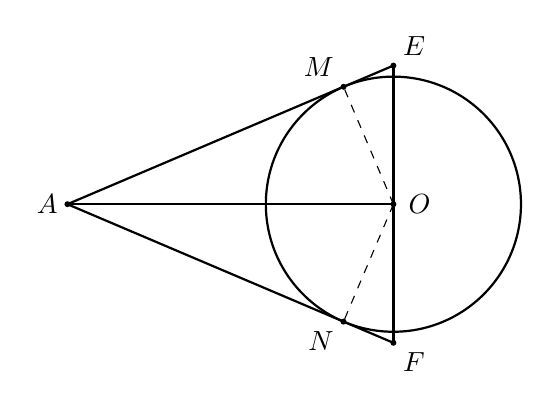
\begin{tikzpicture}[scale=0.9]
  \draw[thick] (0,0) circle (1.8);
  \coordinate (O) at (0,0);
  \coordinate (A) at (-4.6,0);
  \coordinate (M) at (-0.704,1.657);
  \coordinate (N) at (-0.704,-1.657);
  \coordinate (E) at (0,1.956);
  \coordinate (F) at (0,-1.956);
  \draw[thick] (A) -- (E);
  \draw[thick] (A) -- (F);
  \draw[thick] (A) -- (O);
  \draw[thick] (E) -- (F);
  \draw[dashed] (O) -- (M);
  \draw[dashed] (O) -- (N);
  \fill (O) circle (1.2pt) node[right=2pt] {$O$};
  \fill (A) circle (1.2pt) node[left] {$A$};
  \fill (M) circle (1.2pt) node[above left] {$M$};
  \fill (N) circle (1.2pt) node[below left] {$N$};
  \fill (E) circle (1.2pt) node[above right] {$E$};
  \fill (F) circle (1.2pt) node[below right] {$F$};
\end{tikzpicture}
\end{center}
\nopagebreak[4]
\Needspace{0.4\textheight}
\end{question}
\begin{question}
\gkti{7}如果平面内一动点 $P$ 到点 $(-4,\ 0)$ 的距离等于它到直线 $x=-\dfrac{25}{4}$ 的距离的 $\dfrac{4}{5}$，求 $P$ 点的轨迹方程，又这是一条什么曲线？

\Needspace{5\baselineskip}
\textbf{参考题 1．} 方程组

\nopagebreak[4]
\[
\begin{cases}
x_1+3x_2+2x_3-x_4=1,\\
x_2-2x_3+x_4=-1,\\
2x_1+x_3+2x_4=0,\\
2x_2+ax_3-2x_4=1
\end{cases}
\]

中，当 $a$ 取什么值时，该方程组有解？（有多少组解？）又当 $a$ 取什么值时，方程组无解？

\textbf{参考题 2．} 有一份印刷品，其排版面积（矩形）占 $432$ 平方厘米，它的两边都留有 $4$ 厘米宽的空白，顶部和底部留有 $3$ 厘米宽的空白。问应该如何选取纸张的尺寸，才能使纸的用量最少？

\begin{gktip}
原源 PDF 第 5 页附有纸张与排版面的示意图；LaTeX 版按源图重绘。
\end{gktip}
\nopagebreak[4]
\begin{center}% 1977 年广东卷参考题 2：纸张矩形（左右长 x、上下宽 y），内阴影矩形为排版面 432，
% 左右边距 4 厘米、上下边距 3 厘米（按源卷第 5 页布局）
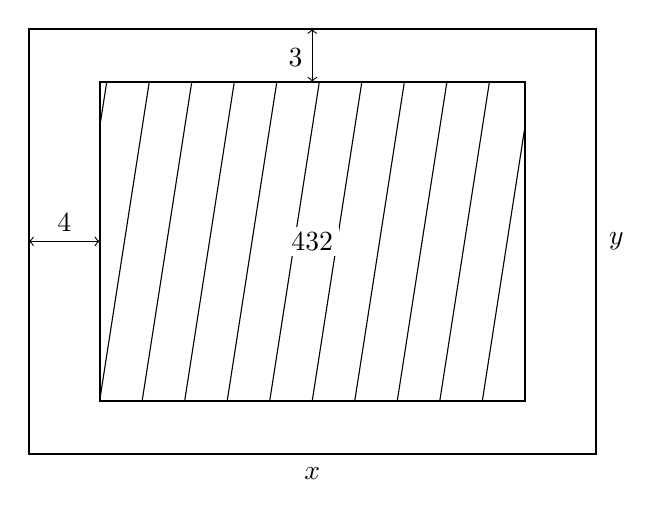
\begin{tikzpicture}[scale=0.9]
  \draw[thick] (0,0) rectangle (8,6);
  \begin{scope}
    \clip (1,0.75) rectangle (7,5.25);
    \foreach \i in {-7,...,10}
      \draw (1+\i*0.6,0.75) -- (1.7+\i*0.6,5.25);
  \end{scope}
  \draw[thick] (1,0.75) rectangle (7,5.25);
  \node[fill=white,inner sep=2pt] at (4,3) {$432$};
  % 边距标注
  \draw[<->] (0,3) -- (1,3);
  \node[above] at (0.5,3) {$4$};
  \draw[<->] (4,5.25) -- (4,6);
  \node[left] at (4,5.6) {$3$};
  % 纸张尺寸标注
  \node[below] at (4,-0.05) {$x$};
  \node[right] at (8.05,3) {$y$};
\end{tikzpicture}
\end{center}
\nopagebreak[4]

\end{question}